\chapter{Deployment, Cloud Hosting, and Local Startup Operations}

\section{Introduction}
A major challenge when developing full-stack university software projects is hosting costs. Commercial cloud providers often incur substantial monthly expenses for virtual machines, managed databases, and edge gateways. For StayMart, our goal was to architect a \textbf{production-ready, 100\% free-tier cloud deployment topology} that enables students, evaluators, and independent developers to deploy and operate the entire platform without incurring server bills.

StayMart is engineered to run seamlessly across two target environments:
\begin{enumerate}
    \item \textbf{Free-Tier Production Cloud Topology:} A decoupled cloud setup combining Vercel for static edge CDN hosting and reverse proxying, Render or Koyeb for containerized Spring Boot and Flask microservices, and TiDB Serverless for managed MySQL persistence.
    \item \textbf{Local Development Environment:} A lightweight local setup using Docker for MySQL, native Maven compilation, and a Python virtual environment, orchestrated via a single PowerShell startup script.
\end{enumerate}

\section{Free-Tier Production Cloud Hosting Topology}
The production cloud topology decouples the system into four zero-cost tiers, eliminating single points of failure while respecting free-tier memory and compute constraints.

\begin{figure}[htbp]
    \centering
    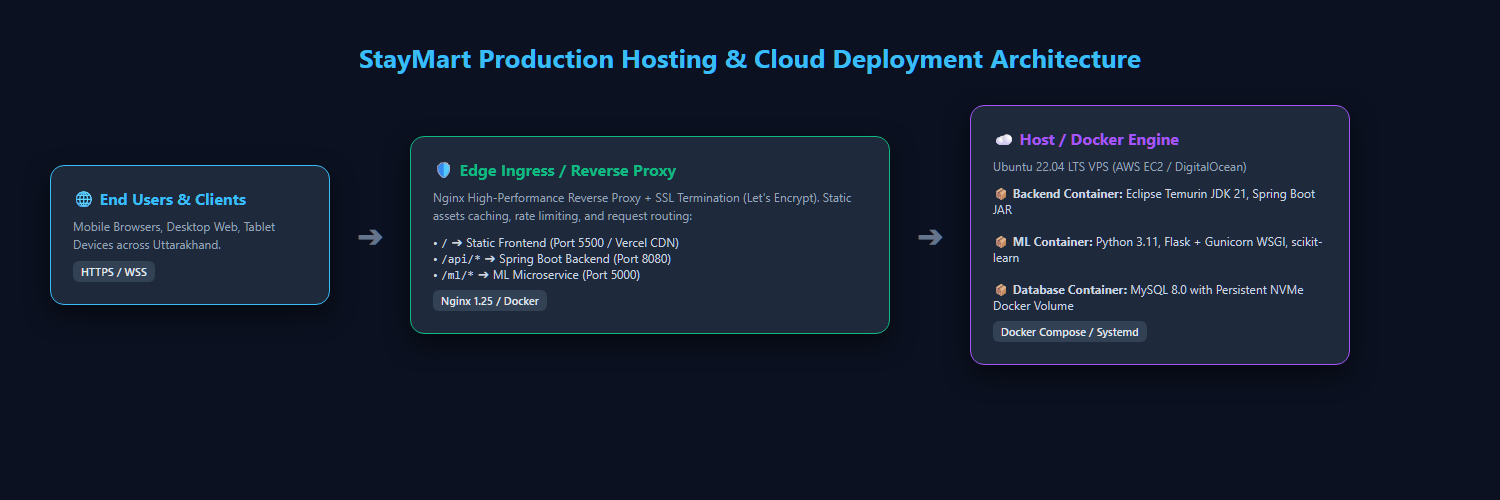
\includegraphics[width=0.95\textwidth]{diagrams/deployment_arch.png}
    \caption{StayMart Production Cloud Hosting Topology Across Free-Tier Providers}
    \label{fig:prod_cloud_arch}
\end{figure}

The four tiers operate as follows:
\begin{itemize}
    \item \textbf{Tier 1: Static Edge CDN (Vercel):} The vanilla HTML5/CSS3/JavaScript frontend is deployed to Vercel's global edge network. Vercel automatically provides HTTPS SSL certificates, global CDN caching, and sub-20ms Time-to-First-Byte (TTFB). Reverse proxy rewrite rules in \texttt{vercel.json} route all \texttt{/api/*} calls directly to the Spring Boot backend, completely avoiding Cross-Origin Resource Sharing (CORS) complexities in production.
    \item \textbf{Tier 2: Core REST Backend Service (Render / Koyeb Free Tier):} The Spring Boot 3.3 backend runs in a containerized Linux environment under Java 17 LTS. To ensure reliable execution within the 512 MB RAM limit of free cloud containers, the JVM is configured with strict memory guardrails: \texttt{-Xmx384m -XX:+UseSerialGC}. This prevents the Linux Out-of-Memory (OOM) killer from terminating the container during peak traffic.
    \item \textbf{Tier 3: Machine Learning Microservice (Render / Koyeb Free Tier):} The Python 3.11 / Flask recommendation microservice runs as an independent container. It provides a lightweight \texttt{GET /health} endpoint used for health checks and keep-alive monitoring. If the free-tier container experiences a cold start, the Spring Boot backend's 2000ms timeout seamlessly falls back to database-driven recommendations without disrupting the user.
    \item \textbf{Tier 4: Managed Cloud Database (TiDB Serverless / Aiven Free Tier):} The relational database is hosted on TiDB Serverless, which provides 5 GB of free storage forever with MySQL 8.0 wire compatibility, automated daily backups, and encrypted connections enforced via TLS/SSL (\texttt{useSSL=true}).
\end{itemize}

\section{Multi-Service Containerization and Docker Configurations}
To guarantee reproducible builds between development and cloud production, both backend services are containerized.

\subsection{Spring Boot Multi-Stage Dockerfile}
Listing \ref{lst:dockerfile_backend} presents the production multi-stage \texttt{Dockerfile} located at the project root. It compiles the application in a temporary Maven image and packages the executable JAR into an optimized Java 17 runtime container.

\begin{lstlisting}[language=bash, caption={Multi-Stage Dockerfile for Spring Boot Backend}, label={lst:dockerfile_backend}]
# Stage 1: Build stage
FROM maven:3.9.6-eclipse-temurin-17 AS build
WORKDIR /app
COPY pom.xml .
RUN mvn dependency:go-offline -B
COPY src ./src
RUN mvn clean package -DskipTests

# Stage 2: Runtime stage
FROM eclipse-temurin:17-jre-jammy
WORKDIR /app
COPY --from=build /app/target/staymart-*.jar app.jar
ENV PORT=8080
ENV JAVA_OPTS="-Xmx384m -XX:+UseSerialGC"
EXPOSE 8080
ENTRYPOINT ["sh", "-c", "java $JAVA_OPTS -Dserver.port=${PORT} -jar app.jar"]
\end{lstlisting}

\subsection{Python Flask ML Microservice Dockerfile}
Listing \ref{lst:dockerfile_ml} details the lightweight container configuration for the recommendation microservice located at \texttt{ml-service/Dockerfile}:

\begin{lstlisting}[language=bash, caption={Lightweight Dockerfile for ML Microservice (ml-service/Dockerfile)}, label={lst:dockerfile_ml}]
FROM python:3.11-slim
WORKDIR /app

# Install system build dependencies and scikit-learn requirements
RUN apt-get update && apt-get install -y --no-install-recommends \
    gcc g++ && \
    rm -rf /var/lib/apt/lists/*

COPY requirements.txt .
RUN pip install --no-cache-dir -r requirements.txt

COPY . .
ENV PORT=5000
EXPOSE 5000

CMD ["python", "app.py"]
\end{lstlisting}

\subsection{Local Development Docker Compose}
For developers running all services locally, Listing \ref{lst:docker_compose} provides a local \texttt{docker-compose.yml} configuration:

\begin{lstlisting}[language=XML, caption={Local docker-compose.yml Configuration}, label={lst:docker_compose}]
version: '3.8'

services:
  mysql:
    image: mysql:8.0
    container_name: staymart-mysql
    restart: always
    environment:
      MYSQL_ROOT_PASSWORD: root
      MYSQL_DATABASE: staymart
    ports:
      - "3306:3306"
    volumes:
      - mysql_data:/var/lib/mysql
      - ./database/01_schema.sql:/docker-entrypoint-initdb.d/01_schema.sql:ro
      - ./database/02_seed.sql:/docker-entrypoint-initdb.d/02_seed.sql:ro
      - ./database/03_seed_listings.sql:/docker-entrypoint-initdb.d/03_seed_listings.sql:ro
    healthcheck:
      test: ["CMD", "mysqladmin", "ping", "-h", "localhost"]
      interval: 10s
      timeout: 5s
      retries: 5

volumes:
  mysql_data:
\end{lstlisting}

\section{Edge Routing and Reverse Proxy Rewrites}
In traditional enterprise setups, an Nginx reverse proxy handles routing and SSL certificates. In StayMart's zero-cost cloud architecture, edge routing is handled directly by Vercel via \texttt{vercel.json}:

\begin{lstlisting}[language=XML, caption={Vercel Edge Reverse Proxy Configuration (vercel.json)}]
{
  "version": 2,
  "rewrites": [
    {
      "source": "/api/(.*)",
      "destination": "https://staymart-backend.onrender.com/api/$1"
    },
    {
      "source": "/",
      "destination": "/frontend/index.html"
    },
    {
      "source": "/(.*)",
      "destination": "/frontend/$1"
    }
  ]
}
\end{lstlisting}

This setup routes all frontend requests directly to cached HTML/CSS/JS files, while requests to \texttt{/api/*} are forwarded transparently to the Spring Boot cloud backend. For developers who prefer self-hosting on a dedicated Linux VPS, an alternative Nginx configuration with Let's Encrypt SSL can also be used.

\section{Static Edge Hosting with Vercel}
Deploying the frontend to Vercel requires no build scripts:
\begin{enumerate}
    \item Install the Vercel CLI: \texttt{npm i -g vercel}
    \item Deploy from the project root: \texttt{vercel deploy --prod}
    \item Vercel reads \texttt{vercel.json}, sets up HTTPS automatically, and deploys the static files to its global CDN.
\end{enumerate}

\section{Local Startup and Development Runbook}
To make testing and evaluation seamless, StayMart provides both automated scripts and manual startup procedures.

\subsection{One-Command Automated Startup (Windows PowerShell)}
The script \texttt{scripts/start-all.ps1} starts the complete ecosystem:
\begin{lstlisting}[language=bash]
pwsh -File scripts/start-all.ps1
\end{lstlisting}

The script automates the following steps:
\begin{enumerate}
    \item Checks Docker daemon status and boots the \texttt{staymart-mysql} container on port 3306.
    \item Verifies schema tables and applies seed scripts if the database is newly created.
    \item Confirms Java 17+ (or system JDK), compiles backend code, and launches Spring Boot on port 8080.
    \item Activates the Python virtual environment and launches the Flask ML microservice on port 5000.
    \item Starts a local Python HTTP server on port 5500 serving the frontend.
\end{enumerate}
To gracefully stop all background services:
\begin{lstlisting}[language=bash]
pwsh -File scripts/stop-all.ps1
\end{lstlisting}

\subsection{Manual Step-by-Step Startup (macOS / Linux / Windows)}
Developers who prefer manual terminal commands can execute the following:

\textbf{Step 1: Start MySQL Database}
\begin{lstlisting}[language=bash]
docker run --name staymart-mysql -e MYSQL_ROOT_PASSWORD=root -e MYSQL_DATABASE=staymart -p 3306:3306 -d mysql:8.0
mysql -h 127.0.0.1 -u root -proot staymart < database/01_schema.sql
mysql -h 127.0.0.1 -u root -proot staymart < database/02_seed.sql
mysql -h 127.0.0.1 -u root -proot staymart < database/03_seed_listings.sql
\end{lstlisting}

\textbf{Step 2: Start Spring Boot Core Backend}
\begin{lstlisting}[language=bash]
mvn clean package -DskipTests
mvn spring-boot:run
# Backend initializes at http://localhost:8080/api
\end{lstlisting}

\textbf{Step 3: Start Python ML Microservice}
\begin{lstlisting}[language=bash]
cd ml-service
python -m venv .venv
source .venv/bin/activate       # On Windows: .venv\Scripts\activate
pip install -r requirements.txt
python app.py                   # Starts microservice at http://localhost:5000
\end{lstlisting}

\textbf{Step 4: Serve Frontend Web Application}
\begin{lstlisting}[language=bash]
cd frontend
python -m http.server 5500
# Open browser at http://localhost:5500
\end{lstlisting}

\section{Continuous Integration with GitHub Actions}
Listing \ref{lst:github_actions} details the automated GitHub Actions workflow (\texttt{.github/workflows/ci.yml}) verifying compilation and test suites on every pull request.

\begin{lstlisting}[language=XML, caption={GitHub Actions CI Pipeline (.github/workflows/ci.yml)}, label={lst:github_actions}]
name: StayMart CI Pipeline

on:
  push:
    branches: [ main, develop ]
  pull_request:
    branches: [ main ]

jobs:
  backend-build:
    runs-on: ubuntu-latest
    services:
      mysql:
        image: mysql:8.0
        env:
          MYSQL_ROOT_PASSWORD: root
          MYSQL_DATABASE: staymart
        ports:
          - 3306:3306
        options: --health-cmd="mysqladmin ping" --health-interval=10s --health-timeout=5s --health-retries=3

    steps:
      - uses: actions/checkout@v3

      - name: Set up JDK 17
        uses: actions/setup-java@v3
        with:
          java-version: '17'
          distribution: 'temurin'
          cache: maven

      - name: Build with Maven
        run: mvn clean verify -B

  ml-test:
    runs-on: ubuntu-latest
    steps:
      - uses: actions/checkout@v3

      - name: Set up Python 3.11
        uses: actions/setup-python@v4
        with:
          python-version: '3.11'

      - name: Install ML Dependencies
        run: |
          cd ml-service
          python -m pip install --upgrade pip
          pip install -r requirements.txt

      - name: Test Syntax Compilation
        run: |
          cd ml-service
          python -m py_compile app.py recommender.py config.py
\end{lstlisting}

\section{Summary}
This chapter presented the deployment architecture and operational workflows for StayMart. We detailed the 100\% free-tier cloud deployment topology combining Vercel, Render/Koyeb, and TiDB Serverless. We provided multi-stage Dockerfile specifications with JVM memory guardrails (\texttt{-Xmx384m}), documented reverse proxy rewrites, and provided local orchestration scripts. The final chapter reviews the project's milestones, lessons learned, and future technical roadmap.
